
%%%
% Any results of the experimental runs
%%%

\subsection{Further Experiments}
\label{sec:findings-expts}

%%%
As the results of Round 2 emulated those of Round 1,
additional modifications were applied to the learning process.
%
These methods focused on directly affecting the weights applied to each
decision made,
both in learning and at choosing time.
%
The intended goal of these modifications were to find a policy
capable of learning a policy which plays the game consistently better than
random.
%
All modifications for these experiments started with the following common
parameters:
\begin{itemize}
	\item Scaling Factor: $s = 2.0$
	\item Decay: $d = 0.1$
	\item Random Exploration Chance: $e = 0.3$
\end{itemize}
%
Additionally,
the pegging records database was standardized across all experiments
as one selected from those resulting from the first round of training.
%
As a final note,
the mechanism for choosing a combination of cards using the \pvec\ vector 
during the tournament was altered slightly.
%
As previously mentioned,
when making an exploration step,
instead of using \pvec\ as a probability distribution,
the choice was made at uniform random,
in a manner true to $\epsilon$-greedy exploration~\cite{rl_book}.
%
This was done for the sake of simplicity.
%
Furthermore,
the difference in choosing mechanisms demonstrably
made no noticeable difference in the learning behavior,
perhaps as a result of \pvec\ being near-uniformly random for untrained states
and in essence a choice between three or four most desirable choices when
states had been visited.
%%%

%
%%%
% Explanation of round-robin structure and why it was done
%%%

\subsubsection*{Round-Robin Play}
\label{sec:findings-expts-rr}

%%%
Since the agents were deemed to be learning to outplay each other,
but not necessarily how to optimally play the game,
training against a single opponent for a million games was determined to be
an issue.
%
To determine how tailoring play to a single opponent affected the final outcome
weights,
a round-robin structure was implemented in which multiple agents would swap out
opponents occasionally.
%
Given a pool of potential agents,
every $N$ games,
a random pair of agents are selected from the pool and played against one
another.
%
By varying opponents every so often,
the intention of the round-robin structure should eliminate an agent's
dependence on another's strategy for performance.
%%%




%%%
% Discuss how neighboring weights were applied and what the results were
%%%

\subsubsection*{Neighboring Weights}
\label{sec:findings-expts-neighbors}

%%%
% Process
%%%

%%%
In order to smooth out the strategy graphs
and prevent isolated states of separate weights,
a blending of neighboring weights was developed.
%
Rather than simply take the set of weights allocated to a single score location,
the agent instead takes a weighted average of all surrounding weight vectors
with its own location.
%
In other words,
\[
    \wvecm'_{p,o,d} = %\mathrm{l1norm}\left(
    \left|
    X\wvecm_{p,o,d} +
    Y \sum_{i\in\{-1,0,1\}} \sum_{j\in\{-1,0,1\}} \wvecm_{p+i,o+j,d}
    \right|_1
    %\right)
\]
where $X$, $Y$ are ratios of each vector's effect, $X+Y = 1$,
and $p+i$, $o+j \in [0,120]$.
%
The desired effect was to allow a score location to learn from its neighbors
so that an area effect was present in the decision.
%%%


\paragraph*{Results}

%%%
% Results:
%	Mostly same appearnace
%	fewer islands in hand_max_min territory for cribminavg/peggingminavggiven/
%		peggingmaxmedgained/peggingmaxavggained
%	Losing territory still in limbo, not much certainty there.
%%%

%%%
% Not really good at making a blending/gradient
% Definitely did eliminate islands though
%%%


\begin{figure}
\center

	\begin{subfigure}[t]{0.22\textwidth}
		\center
		
\includegraphics[width=\stratgraphwidth]{images/findings/experiments/neighbors/strats/hand_max_min.png}
		\caption{\handmaxmin}
	\end{subfigure}
	~
	\begin{subfigure}[t]{0.22\textwidth}
		\center
		
\includegraphics[width=\stratgraphwidth]{images/findings/experiments/neighbors/strats/hand_max_avg.png}
		\caption{\handmaxavg}
	\end{subfigure}
~
	\begin{subfigure}[t]{0.22\textwidth}
		\center
		
\includegraphics[width=\stratgraphwidth]{images/findings/experiments/neighbors/strats/hand_max_med.png}
		\caption{\handmaxmed}
	\end{subfigure}
	~
	\begin{subfigure}[t]{0.22\textwidth}
		\center
		
\includegraphics[width=\stratgraphwidth]{images/findings/experiments/neighbors/strats/hand_max_poss.png}
		\caption{\handmaxposs}
	\end{subfigure}

	\begin{subfigure}[t]{0.22\textwidth}
		\center
		
\includegraphics[width=\stratgraphwidth]{images/findings/experiments/neighbors/strats/crib_min_avg.png}
		\caption{\cribminavg}
	\end{subfigure}
	~
	\begin{subfigure}[t]{0.22\textwidth}
		\center
		
\includegraphics[width=\stratgraphwidth]{images/findings/experiments/neighbors/strats/pegging_max_avg_gained.png}
		\caption{\peggingmaxavggained}
	\end{subfigure}
~
	\begin{subfigure}[t]{0.22\textwidth}
		\center
		
\includegraphics[width=\stratgraphwidth]{images/findings/experiments/neighbors/strats/pegging_max_med_gained.png}
		\caption{\peggingmaxmedgained}
	\end{subfigure}
	~
	\begin{subfigure}[t]{0.22\textwidth}
		\center
		
\includegraphics[width=\stratgraphwidth]{images/findings/experiments/neighbors/strats/pegging_min_avg_given.png}
		\caption{\peggingminavggiven}
	\end{subfigure}

\caption{
	Final strategy graphs for an agent when playing as the dealer
	after being trained for 500,000 games
	by following a policy which uses a weighted sum of neighboring weights.
}
\label{fig:neighbor-strats}
\end{figure}


%%%
The agent was not
able to develop gradient-like strategy graphs
using the neighborhood technique.
%
In fact,
the \handmaxavg\ strategy,
which one would most expect to form a gradient with and around the
\handmaxmin\ strategy,
was perhaps the most negatively affected.
%
As seen in Figure~\ref{fig:neighbor-strats},
the \handmaxavg\ strategy graph has become more sparse in the winning
states (lower left)
with very little gray area surrounding the black.
%
However,
the presence of gray
indicates that a melding of strategies did occur.
%%%

%%%
Interestingly,
while the neighboring weights did not solidify any presence in the graphs,
the new training method did make progress in negative space.
%
This is to say that
the weighted neighbors learning method eliminated the usually present islands
of a single strategy within a swathe of another dominant strategy.
%
This white-space was present in both the winning and losing states.
%
This finding leads to the conclusion that weighted learning techniques
do indeed allow for a sharing of knowledge between like states,
but only insofar as to know what not to do.
%%%

%%%
Furthermore,
there is still a vast degree of uncertainty present in the losing states of
the strategy graphs.
%
The theory that the certainty of the winning states might potentially
bleed over into the losing side was not demonstrated over the course of
the first half million training games.
%
However,
since the elimination of islands shows an improvement in
preventing lucky happenstance to dictate a space's future,
the neighboring weights training method has shown usefulness in training a
cribbage agent in which states neighboring states are often similar in nature.
%%%




%%%
% Regularization to prevent too strong of weights
%%%

\subsubsection*{Regularization}

%%%
% Process
%%%

%%%
As an attempt to prevent a single strategy's weight from being so strongly 
preferred that a second strategy could not hope to possibly gain ground,
a hard limit was placed on the pre-normalized update value.
%
Expressed mathematically,
\[
    \wvecm'_{p,o,d}[i] = \max\{K,c\wvecm_{p,o,d}[i]\}
\]
where $K$ is some constant value throughout the training.
%
While the value of $w_{m,o,d}[i]$ could exceed $K$ after re-normalization
for a particularly strongly weighted strategy,
the value could be seen converging to $K$ within just a handful of iterations.
%
The desired intention of this regularization was to allow other strategies
the opportunity to overcome the bias of earlier strengthening of the strongest
strategy.
%%%

\paragraph*{Results}

%%%
% Results:
%	Similar areas taken up for hand_max_{min,avg}
%		both share same space rather than Croatia/Boz&Herz-shape
%	Grayer, since values only so large
%	As max value is increased,
%		darker, more like un-regulated
%	Islands still present
%	losing, still uncertain
%		still chance of higher than regulation, because of aforementioned reason
%%%


\begin{figure}
\center

	\begin{subfigure}[t]{0.22\textwidth}
		\center
		
\includegraphics[width=\textwidth]{images/findings/experiments/regularization/strats/0.50/hand_max_min.png}
		\caption{\handmaxmin}
	\end{subfigure}
	~
	\begin{subfigure}[t]{0.22\textwidth}
		\center
		
\includegraphics[width=\textwidth]{images/findings/experiments/regularization/strats/0.50/hand_max_avg.png}
		\caption{\handmaxavg}
	\end{subfigure}
~
	\begin{subfigure}[t]{0.22\textwidth}
		\center
		
\includegraphics[width=\textwidth]{images/findings/experiments/regularization/strats/0.50/hand_max_med.png}
		\caption{\handmaxmed}
	\end{subfigure}
	~
	\begin{subfigure}[t]{0.22\textwidth}
		\center
		
\includegraphics[width=\textwidth]{images/findings/experiments/regularization/strats/0.50/hand_max_poss.png}
		\caption{\handmaxposs}
	\end{subfigure}

	\begin{subfigure}[t]{0.22\textwidth}
		\center
		
\includegraphics[width=\textwidth]{images/findings/experiments/regularization/strats/0.50/crib_min_avg.png}
		\caption{\cribminavg}
	\end{subfigure}
	~
	\begin{subfigure}[t]{0.22\textwidth}
		\center
		
\includegraphics[width=\textwidth]{images/findings/experiments/regularization/strats/0.50/pegging_max_avg_gained.png}
		\caption{\peggingmaxavggained}
	\end{subfigure}
~
	\begin{subfigure}[t]{0.22\textwidth}
		\center
		
\includegraphics[width=\textwidth]{images/findings/experiments/regularization/strats/0.50/pegging_max_med_gained.png}
		\caption{\peggingmaxmedgained}
	\end{subfigure}
	~
	\begin{subfigure}[t]{0.22\textwidth}
		\center
		
\includegraphics[width=\textwidth]{images/findings/experiments/regularization/strats/0.50/pegging_min_avg_given.png}
		\caption{\peggingminavggiven}
	\end{subfigure}

\caption{
	Final strategies for an agent using regularized learning
	when playing as the pone
	and the maximum value weight allowed is 0.50
	after training for 500,000 games.
}
\label{fig:reg-strats-0.50}
\end{figure}

%
\begin{figure}
\center

	\begin{subfigure}[t]{0.22\textwidth}
		\center
		
\includegraphics[width=\textwidth]{images/findings/experiments/regularization/strats/0.60/hand_max_min.png}
		\caption{\handmaxmin}
	\end{subfigure}
	~
	\begin{subfigure}[t]{0.22\textwidth}
		\center
		
\includegraphics[width=\textwidth]{images/findings/experiments/regularization/strats/0.60/hand_max_avg.png}
		\caption{\handmaxavg}
	\end{subfigure}
~
	\begin{subfigure}[t]{0.22\textwidth}
		\center
		
\includegraphics[width=\textwidth]{images/findings/experiments/regularization/strats/0.60/hand_max_med.png}
		\caption{\handmaxmed}
	\end{subfigure}
	~
	\begin{subfigure}[t]{0.22\textwidth}
		\center
		
\includegraphics[width=\textwidth]{images/findings/experiments/regularization/strats/0.60/hand_max_poss.png}
		\caption{\handmaxposs}
	\end{subfigure}

	\begin{subfigure}[t]{0.22\textwidth}
		\center
		
\includegraphics[width=\textwidth]{images/findings/experiments/regularization/strats/0.60/crib_min_avg.png}
		\caption{\cribminavg}
	\end{subfigure}
	~
	\begin{subfigure}[t]{0.22\textwidth}
		\center
		
\includegraphics[width=\textwidth]{images/findings/experiments/regularization/strats/0.60/pegging_max_avg_gained.png}
		\caption{\peggingmaxavggained}
	\end{subfigure}
~
	\begin{subfigure}[t]{0.22\textwidth}
		\center
		
\includegraphics[width=\textwidth]{images/findings/experiments/regularization/strats/0.60/pegging_max_med_gained.png}
		\caption{\peggingmaxmedgained}
	\end{subfigure}
	~
	\begin{subfigure}[t]{0.22\textwidth}
		\center
		
\includegraphics[width=\textwidth]{images/findings/experiments/regularization/strats/0.60/pegging_min_avg_given.png}
		\caption{\peggingminavggiven}
	\end{subfigure}

\caption{
	Final strategies for an agent using regularized learning
	when playing as the dealer
	and the maximum value weight allowed is 0.60
	after training for 500,000 games.
}
\label{fig:neighbor-strats}
\end{figure}

%
\begin{figure}
\center

	\begin{subfigure}[t]{0.22\textwidth}
		\center
		
\includegraphics[width=\textwidth]{images/findings/experiments/regularization/strats/0.70/hand_max_min.png}
		\caption{\handmaxmin}
	\end{subfigure}
	~
	\begin{subfigure}[t]{0.22\textwidth}
		\center
		
\includegraphics[width=\textwidth]{images/findings/experiments/regularization/strats/0.70/hand_max_avg.png}
		\caption{\handmaxavg}
	\end{subfigure}
~
	\begin{subfigure}[t]{0.22\textwidth}
		\center
		
\includegraphics[width=\textwidth]{images/findings/experiments/regularization/strats/0.70/hand_max_med.png}
		\caption{\handmaxmed}
	\end{subfigure}
	~
	\begin{subfigure}[t]{0.22\textwidth}
		\center
		
\includegraphics[width=\textwidth]{images/findings/experiments/regularization/strats/0.70/hand_max_poss.png}
		\caption{\handmaxposs}
	\end{subfigure}

	\begin{subfigure}[t]{0.22\textwidth}
		\center
		
\includegraphics[width=\textwidth]{images/findings/experiments/regularization/strats/0.70/crib_min_avg.png}
		\caption{\cribminavg}
	\end{subfigure}
	~
	\begin{subfigure}[t]{0.22\textwidth}
		\center
		
\includegraphics[width=\textwidth]{images/findings/experiments/regularization/strats/0.70/pegging_max_avg_gained.png}
		\caption{\peggingmaxavggained}
	\end{subfigure}
~
	\begin{subfigure}[t]{0.22\textwidth}
		\center
		
\includegraphics[width=\textwidth]{images/findings/experiments/regularization/strats/0.70/pegging_max_med_gained.png}
		\caption{\peggingmaxmedgained}
	\end{subfigure}
	~
	\begin{subfigure}[t]{0.22\textwidth}
		\center
		
\includegraphics[width=\textwidth]{images/findings/experiments/regularization/strats/0.70/pegging_min_avg_given.png}
		\caption{\peggingminavggiven}
	\end{subfigure}

\caption{
	Final strategies for an agent using regularized learning
	when playing as the pone
	and the maximum value weight allowed is 0.70
	after training for 500,000 games.
}
\label{fig:reg-strats-0.70}
\end{figure}


\begin{figure}
\center

	\begin{subfigure}[t]{0.22\textwidth}
		\center
		
\includegraphics[width=\textwidth]{images/findings/experiments/regularization/strats/0.80/hand_max_min.png}
		\caption{\handmaxmin}
	\end{subfigure}
	~
	\begin{subfigure}[t]{0.22\textwidth}
		\center
		
\includegraphics[width=\textwidth]{images/findings/experiments/regularization/strats/0.80/hand_max_avg.png}
		\caption{\handmaxavg}
	\end{subfigure}
~
	\begin{subfigure}[t]{0.22\textwidth}
		\center
		
\includegraphics[width=\textwidth]{images/findings/experiments/regularization/strats/0.80/hand_max_med.png}
		\caption{\handmaxmed}
	\end{subfigure}
	~
	\begin{subfigure}[t]{0.22\textwidth}
		\center
		
\includegraphics[width=\textwidth]{images/findings/experiments/regularization/strats/0.80/hand_max_poss.png}
		\caption{\handmaxposs}
	\end{subfigure}

	\begin{subfigure}[t]{0.22\textwidth}
		\center
		
\includegraphics[width=\textwidth]{images/findings/experiments/regularization/strats/0.80/crib_min_avg.png}
		\caption{\cribminavg}
	\end{subfigure}
	~
	\begin{subfigure}[t]{0.22\textwidth}
		\center
		
\includegraphics[width=\textwidth]{images/findings/experiments/regularization/strats/0.80/pegging_max_avg_gained.png}
		\caption{\peggingmaxavggained}
	\end{subfigure}
~
	\begin{subfigure}[t]{0.22\textwidth}
		\center
		
\includegraphics[width=\textwidth]{images/findings/experiments/regularization/strats/0.80/pegging_max_med_gained.png}
		\caption{\peggingmaxmedgained}
	\end{subfigure}
	~
	\begin{subfigure}[t]{0.22\textwidth}
		\center
		
\includegraphics[width=\textwidth]{images/findings/experiments/regularization/strats/0.80/pegging_min_avg_given.png}
		\caption{\peggingminavggiven}
	\end{subfigure}

\caption{
	Final strategies for an agent using regularized learning
	when playing as the dealer
	and the maximum value weight allowed is 0.80
	after training for 500,000 games.
}
\label{fig:reg-strats-0.80}
\end{figure}


\begin{figure}
\centering

	\begin{tabular}{l l p{2.75cm} p{2.75cm} p{2.75cm} p{2.75cm}}
	& & \multicolumn{4}{c}{\textit{Regularization Rate}} \\
	&
		& $r = 0.5$
		& $r = 0.6$
		& $r = 0.7$
		& $r = 0.8$
		\\
	%
	\multirow{2}{*}{
	\rotatebox{90}{
	\parbox[c]{2.5cm}{
		\textit{Strategy}
	}
	}
	}
	%
	& \rotatebox[origin=c]{90}{\handmaxmin}
		&\parbox[c]{1em}{
\includegraphics[width=\stratgraphwidthmed]{images/findings/experiments/regularization/strats/0.50/hand_max_min.png}}
		&\parbox[c]{1em}{
\includegraphics[width=\stratgraphwidthmed]{images/findings/experiments/regularization/strats/0.60/hand_max_min.png}}
		&\parbox[c]{1em}{
\includegraphics[width=\stratgraphwidthmed]{images/findings/experiments/regularization/strats/0.70/hand_max_min.png}}
		&\parbox[c]{1em}{
\includegraphics[width=\stratgraphwidthmed]{images/findings/experiments/regularization/strats/0.80/hand_max_min.png}}
	%
	\\ & & & & & \\
	& \rotatebox[origin=c]{90}{\handmaxavg}
		&\parbox[c]{1em}{
\includegraphics[width=\stratgraphwidthmed]{images/findings/experiments/regularization/strats/0.50/hand_max_avg.png}}
		&\parbox[c]{1em}{
\includegraphics[width=\stratgraphwidthmed]{images/findings/experiments/regularization/strats/0.60/hand_max_avg.png}}
		&\parbox[c]{1em}{
\includegraphics[width=\stratgraphwidthmed]{images/findings/experiments/regularization/strats/0.70/hand_max_avg.png}}
		&\parbox[c]{1em}{
\includegraphics[width=\stratgraphwidthmed]{images/findings/experiments/regularization/strats/0.80/hand_max_avg.png}}
\end{tabular}

\caption{
	Comparison of the \handmaxmin\ and \handmaxavg\ strategies
	for each of the regularization rates ($r$) used
	when the agent is playing as the pone.
}
\label{fig:expts-reg-comp}
\end{figure}



%%%
As was expected,
the limitation of maximum attainable value did indeed force the agent to learn
multiple applicable strategies for each score location.
%
As can be seen in Figure~\ref{fig:reg-strats-0.50},
the \handmaxmin\ and \handmaxavg\ strategies are now 
more or less equally represented across the winning triangle area.
%
This is demonstrated by the monotone gray seen in these locations.
%
Rather than each strategy specializing to its own dominant location,
the territory is shared between the two most applicable strategies.
%
Therefore,
the regularization does indeed prevent the dominance of a single strategy
unintentionally discarding all other potential strategies.
%%%

%%%
Additionally,
the nature of this gray mass alters significantly as the regularization rate is
altered.
%
With a lower allowed maximum value,
the strategy graphs take on the previously mentioned slightly amorphous gray
blob shape.
%
As the maximum value approaches one,
the gray shape begins to specialize more and begins to show resemblance to the
final strategy graphs obtained without regularization.
%
A visualization of this process can be found in
Figure~\ref{fig:expts-reg-comp}.
%%%


\begin{figure}

	\begin{subfigure}[t]{0.48\textwidth}
		\center
		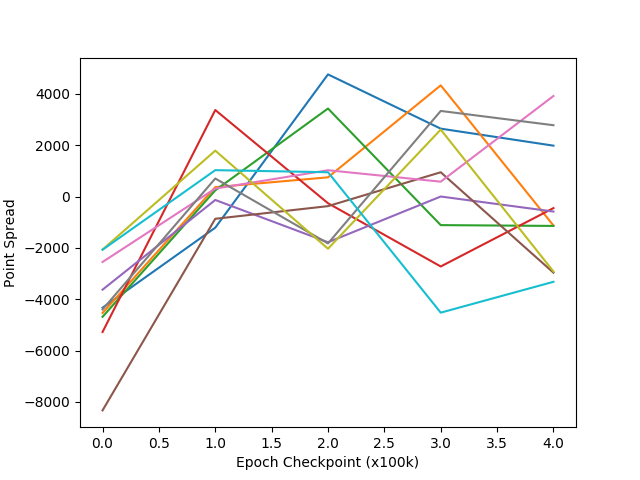
\includegraphics[width=\textwidth]{images/findings/experiments/regularization/tourny/reg_050-kyttuhat-strict-500k.png}
		\caption{$r = 0.50$}
	\end{subfigure}
	~
	\begin{subfigure}[t]{0.48\textwidth}
		\center
		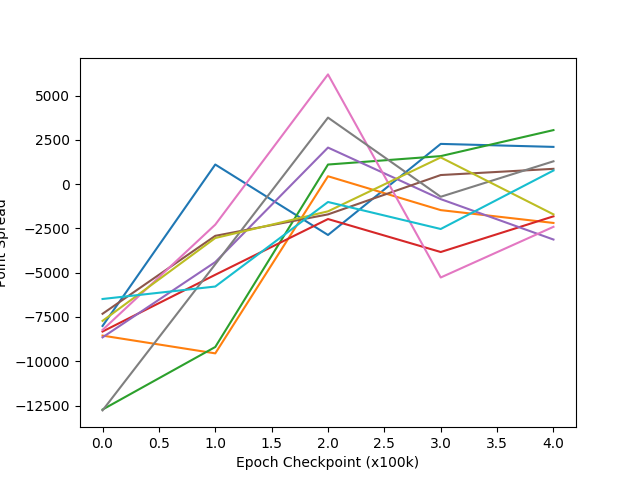
\includegraphics[width=\textwidth]{images/findings/experiments/regularization/tourny/reg_060-kyttuhat-strict-500k.png}
		\caption{$r = 0.60$}
	\end{subfigure}

	\begin{subfigure}[t]{0.48\textwidth}
		\center
		\includegraphics[width=\textwidth]{images/findings/experiments/regularization/tourny/reg_070-kyttuhat-strict-500k.png}
		\caption{$r = 0.70$}
	\end{subfigure}
	~
	\begin{subfigure}[t]{0.48\textwidth}
		\center
		\includegraphics[width=\textwidth]{images/findings/experiments/regularization/tourny/reg_080-kyttuhat-strict-500k.png}
		\caption{$r = 0.80$}
	\end{subfigure}

\caption{
	Point spreads of self-tournaments for 10,000 games
	carried out between agents trained using
	the regulation method mentioned in Section~\ref{sec:findings-r2} after being
	trained for 500,000 games.
	Each tournament plot in n this figure is referenced by the regularization
	rate $r$ in use during training.
}
\label{fig:reg-tournies}
\end{figure}


%%%
Furthermore,
as can be seen in Figure~\ref{fig:reg-tournies},
only a regularization rate of $r = 0.80$ (Figure~\ref{fig:reg-tournies-0.80}
can be said to be similar to a loss curve.
%
With rates of $r=0.50$ (Figure~\ref{fig:reg-tournies-0.50},
$r = 0.60$ (Figure~\ref{fig:reg-tournies-0.60}),
and $r = 0.70$ (Figure~\ref{fig:reg-tournies-0.70}),
the tournament point spread curves show that a trained agent plays on par with
its recent checkpoints,
but consistently worse than random weights.
%
The endpoints of the point spread curves using $r = 0.80$
show a decrease from better-than-random play for the trained agent
to more-or-less on-par performance with its later checkpoints,
indicative of an increase in performance as training progresses.
%
However,
the increases and decreases of performance along the time axis
the wide range of spreads present and the sinusoidal nature of intermediate
checkpoints' spreads
prevents the conclusion that performance is as predictable as that.
%%%




%%%
% Discussion of how each strategy was used as a separate starting point
%%%

\subsubsection{Starting Points}
\label{sec:findings-expts-starts}

%%%
% TODO: vvv
% How data was obtained
% How choices were compared
%%%

%%%
Since a desired outcome of the learning process was to be able to use the
generated strategy graphs to tell how a hand \textit{should} be played in a
certain score position,
a comparison was made between the produced agent and pure strategies
on a database of choices made by humans.
%
There exists a website in which users are prompted with a set of dealt cards and
a given score and must decide which set of cards they would keep in that
specific situation
\cite{dailycribbagehand}.
%%%

%%%
With access to recorded answers,
the agent's choices could be compared to how humans ranked the choice.
%
The retrieved database recorded which responses were given to each query
and could be used to determine how well the agent's choice matched with those
made by humans in the same situation.
%
For each of the more than 3600 usable records,
the choice the agent made was compared against those made by the users of the
website.
%
The results of this comparison can be seen in
Table~\ref{tab:expts-starts-human}. % TODO: ref more tables if created
%%%

%%%
Table~\ref{tab:expts-starts-human} shows that the trained agent chooses the same
set of cards only marginally more often than an agent with randomly allocated
weights.
%
In approximately half of the cases,
the trained agent chooses the same answer as most humans;
in almost 78 percent of the cases,
the answer given by the agent is within the top three most common human answers.
%
Additionally,
most pure strategies,
created by setting their weight to 1 while all others are 0,
performed worse than the trained mixture.
%
Notable exceptions to this trend are the \handmaxposs\ and \handmaxavg\ 
strategies,
suggesting that in more situations than the agent,
the typical human player will play more according to what points can be expected
to be gained from the cut card.
%
Interestingly,
the \handmaxposs\ strategy's presence as the second most common pure strategy
used indicates a significant degree of risk-taking present in the users'
responses.
%%%

%%%
As a result of this finding,
each of these strategies were used as initial weights to the learning process
in order to determine if the agent could learn to fine-tune a policy starting
from a reasonable assertion of good game-play.
%
Since the update mechanism for weights relies upon renormalization of a vector
which as been rewarded or punished,
no modifications would occur in the case of punishment of a pure strategy
since no other weights would have the chance to increase.
%
Therefore,
the pure strategies used before were slightly modified so that each other
element of the $w$ vector would have a small initial value which would be
increased when the pure strategy was punished.
%%%

%%%%%%
%%%It is worth remembering that the data used is collected from users' own
%%%submissions and evaluations as an exercise,
%%%not through actual gameplay.
%%%%
%%%As such,
%%%as evidenced by occasional reading of the forums for each prompt,
%%%the desire to maximize the
%%%%%%


\begin{table}

	\begin{tabular}{|r|c|c|c|p{4cm}|}
		\hline
		\textbf{Strategy} & \textbf{Top 1} & \textbf{Top 2} & \textbf{Top 3}
			& \textbf{Percentage in Top 3 Human Choices} \\
		\hline
		\peggingminavggiven & 160 & 303 & 458 & 12.64 \\\hline
		\peggingmaxmedgained & 268 & 519 & 796 & 21.97 \\\hline
		\peggingmaxavggained & 347 & 650 & 963 & 26.58 \\\hline
		\cribminavg & 380 & 177 & 1081 & 29.84 \\\hline
		\handmaxmin & 1576 & 2288 & 2666 & 73.59 \\\hline
		\textbf{Random} & \textbf{1581} & \textbf{2318} & \textbf{2759} &
			\textbf{76.15} \\\hline
		\handmaxmed & 1649 & 2353 & 2768 & 76.40 \\\hline
		\textbf{Trained} & \textbf{1706} & \textbf{2426} & \textbf{2821} &
			\textbf{77.86} \\\hline
		\handmaxposs & 1677 & 2433 & 2847 & 78.58 \\\hline
		\handmaxavg & 2066 & 2828 & 3168 & 87.44 \\\hline
	\end{tabular}
	% total = 3623
	\caption{
		Number of times the agent using a given strategy chose the same cards as
		the most common choice by human users
		according to 3623 total parsable records obtained from
		\cite{dailycribbagehand}.
		The columns labeled ``Top X'' display the number of times the given
		strategy's choice was within the top X choices of the user base.
		%if at least that many different choices were made
		In this table,
		\textbf{Random} is from the best result of five agents which each used
		independently randomly allocated weights
		and
		\textbf{Trained} uses an agent trained from Round 2 for one million
		games.
	}
	\label{tab:expts-starts-human}
\end{table}





\subsubsection*{Punishment Severity}
\label{sec:findings-expts-punishments}

%%%
Since it was deemed likely that being in a losing position early in the game
tended to never recover and thus result in a loss,
it followed that punishing losing states for something beyond the agent's
control was slightly unfair.
%
Furthermore,
it was postulated that since the punishment mechanism in effect cycled
strategies
and that there was a possibility that an occasionally winning strategy was often
outweighed by the tendency to lose,
a less strict method of punishment could be used to ensure that the occasional
win from a losing position remains visible.
%
As such,
the update step for modifying the weights was adjusted slightly
so that the constant adjustment factor was significantly smaller for losing
games than it was for winning games.
%
Instead of using the adjustment constant of
$C = s \cdot (\text{PlayerScore} - \text{OppScore})$,
for both winning and losing agents,
the losing agent's adjustment factor was defined as
$C = \frac{1}{4} s \cdot (\text{PlayerScore} - \text{OppScore})$.
%%%

\paragraph*{Results}

%%%
The introduction of an amount of forgiveness did not lead to any worthwhile
difference in learned policy.
%
In contrast to the goal of allowing an occasionally good strategy to form
in losing positions,
not unexpectedly,
the losing positions are even less sure as to which strategy to take,
as seen in Figure~\ref{fig:findings-expts-punish-strats}.
%
Therefore,
it may be concluded that the increased likelihood of losing is 
likely not unfairly punishing potentially good recovery policies.
%
It can be argued that $\frac{1}{4}$ was not a proper ratio
to compensate for the likelihood of loss,
but the similarity of patterns learned and decreased certainty
indicate that the punishment mechanism is functioning adequately
%
Similarly,
while reducing the amplitude of changes
does lead to a more gradiented losing policy,
this is effectively the result of a learning rate adjustment.
%
As will be shown in the learning rate experiments,
these forms of adjustments do not lead to differences in learned behaviors.
% TODO: ^^^ really need to verify that learning rate didn't change anything
% for this to be true
%%%

% fig:findings-expts-punish-strats

\begin{figure}
\center

	\begin{subfigure}[t]{0.22\textwidth}
		\includegraphics[width=\textwidth]{images/findings/experiments/punishment/strategies_handmaxmin.png}
		\caption{\handmaxmin}
	\end{subfigure}
	~
	\begin{subfigure}[t]{0.22\textwidth}
		\includegraphics[width=\textwidth]{images/findings/experiments/punishment/strategies_handmaxavg.png}
		\caption{\handmaxavg}
	\end{subfigure}
	~
	\begin{subfigure}[t]{0.22\textwidth}
		\includegraphics[width=\textwidth]{images/findings/experiments/punishment/strategies_handmaxmed.png}
		\caption{\handmaxmed}
	\end{subfigure}
	~
	\begin{subfigure}[t]{0.22\textwidth}
		\includegraphics[width=\textwidth]{images/findings/experiments/punishment/strategies_handmaxposs.png}
		\caption{\handmaxposs}
	\end{subfigure}

	\begin{subfigure}[t]{0.22\textwidth}
		\includegraphics[width=\textwidth]{images/findings/experiments/punishment/strategies_cribminavg.png}
		\caption{\cribminavg}
	\end{subfigure}
	~
	\begin{subfigure}[t]{0.22\textwidth}
		\includegraphics[width=\textwidth]{images/findings/experiments/punishment/strategies_peggingmaxavggained.png}
		\caption{\peggingmaxavggained}
	\end{subfigure}
	~
	\begin{subfigure}[t]{0.22\textwidth}
		\includegraphics[width=\textwidth]{images/findings/experiments/punishment/strategies_peggingmaxmedgained.png}
		\caption{\peggingmaxmedgained}
	\end{subfigure}
	~
	\begin{subfigure}[t]{0.22\textwidth}
		\includegraphics[width=\textwidth]{images/findings/experiments/punishment/strategies_peggingminavggiven.png}
		\caption{\peggingminavggiven}
	\end{subfigure}

\caption{
	Final strategy graphs for an agent which has less severe punishment
	after training for one million games.
}
\label{fig:findings-expts-punish-strats}
\end{figure}





\subsubsection*{Learning Rate Adjustment}
\label{sec:findings-expts-learnrate}

%%%
In order to determine if the learning rate was too high in Round 2,
even though it had been significantly reduced from Round 1,
a varying amount of learning rates were tried.
%
These runs were intended to see if an optimal policy was being overstepped by
making too large of an adjustment.
%%%


\paragraph*{Results}

%%%
% TODO: verify results when experiment has been rerun
% and choose correct set of answers
%%%

%%%
% 2 possibilities foreseeable for results:
%	1. patterns are the same
%	2. something new is learned
%%%


%%%
As can be seen in Figure~\ref{expts-lr-comp},
the same set of behavioral patterns are learned as in previous training
sessions.\footnote{
	As with the decay section,
	this part needs to be rerun,
	so accuracy will need to be verified.
	% TODO: remove footnote
	What's more: since this section is speculative,
	only one of either this paragraph or the next one will actually be used.
}
%
Therefore,
it is safe to speculate that some optimum is not being stepped over,
allowing a worse set of weights to be pursued instead.
%
Thus,
the agent is correctly learning to solve the problem.
%
Ergo,
the problem setup itself or else the system of rewards
must be flawed in some manner.
% TODO: ^ if this is the case, consider opening the sanitycheck section with
% a pointing out of this
%
However,
a decrease in scaling factor leads to slower adjustments,
showing that the scaling factor does indeed function as a learning rate.
%%%

%%%
% TODO: ^ or v: choose one
%%%

%%%
As can be seen in Figure~\ref{expts-lr-comp},
a different set of behavioral patterns are learned when the
scaling factor,
i.e. the learning rate,
is lowered to \${VALUE}. % TODO: <-- value
%
This serves to show that a better policy was previously being skipped over
by previous training sessions.
%
Were time to permit,
this new learning rate would be further trained to find a more optimal
policy.
%
As this is not currently possible,
the results of such an inquiry are left for speculation
or for future research.
% TODO: ^ if this is the case, probably include in discussion section
%%%

% fig:expts-lr-comp
\begin{figure}[h]
	\centering

	\begin{tabular}{c | c c c c}
		% Outline:
		%   s\g |  250k | 500k | 750k | 1mm
		%	0.25
		%   0.50
		%   1.00
		%   1.50
		$s$ \textbf{\textbackslash} game & 250,000 & 500,000 & 750,000 & 1,000,000 \\
		\hline
		\\
		0.25 & % a & b & c & d
			\parbox[c]{5em}{\includegraphics[width=\stratgraphwidthsmall]{images/findings/experiments/learning_rate/lr_025_250.png}} & % 250
			\parbox[c]{5em}{\includegraphics[width=\stratgraphwidthsmall]{images/findings/experiments/learning_rate/lr_025_500.png}} & % 500
			\parbox[c]{5em}{\includegraphics[width=\stratgraphwidthsmall]{images/findings/experiments/learning_rate/lr_025_750.png}} & % 750
			\parbox[c]{5em}{\includegraphics[width=\stratgraphwidthsmall]{images/findings/experiments/learning_rate/lr_025_1mm.png}} \\ % 1mm
		\\
		0.50 & 
			\parbox[c]{5em}{\includegraphics[width=\stratgraphwidthsmall]{images/findings/experiments/learning_rate/lr_050_250.png}} & % 250
			\parbox[c]{5em}{\includegraphics[width=\stratgraphwidthsmall]{images/findings/experiments/learning_rate/lr_050_500.png}} & % 500
			\parbox[c]{5em}{\includegraphics[width=\stratgraphwidthsmall]{images/findings/experiments/learning_rate/lr_050_750.png}} & % 750
			\parbox[c]{5em}{\includegraphics[width=\stratgraphwidthsmall]{images/findings/experiments/learning_rate/lr_050_1mm.png}} \\ % 1mm
		\\
		0.75 & 
			\parbox[c]{5em}{\includegraphics[width=\stratgraphwidthsmall]{images/findings/experiments/learning_rate/lr_075_250.png}} & % 250
			\parbox[c]{5em}{\includegraphics[width=\stratgraphwidthsmall]{images/findings/experiments/learning_rate/lr_075_500.png}} & % 500
			\parbox[c]{5em}{\includegraphics[width=\stratgraphwidthsmall]{images/findings/experiments/learning_rate/lr_075_750.png}} & % 750
			\parbox[c]{5em}{\includegraphics[width=\stratgraphwidthsmall]{images/findings/experiments/learning_rate/lr_075_1mm.png}} \\ % 1mm
		\\
		1.50 & 
			\parbox[c]{5em}{\includegraphics[width=\stratgraphwidthsmall]{images/findings/experiments/learning_rate/lr_150_250.png}} & % 250
			\parbox[c]{5em}{\includegraphics[width=\stratgraphwidthsmall]{images/findings/experiments/learning_rate/lr_150_500.png}} & % 500
			\parbox[c]{5em}{\includegraphics[width=\stratgraphwidthsmall]{images/findings/experiments/learning_rate/lr_150_750.png}} & % 750
			\parbox[c]{5em}{\includegraphics[width=\stratgraphwidthsmall]{images/findings/experiments/learning_rate/lr_150_1mm.png}} \\ % 1mm
	\end{tabular}

\caption{
	Comparison of different scaling factors ($s$),
	learning the \handmaxavg\ strategy
	when playing as the dealer
	over the course of one million games.
	For comparison, $s = 10.0$ and $s = 2.0$ for Rounds 1 and 2, respectively
	(see Figures~\ref{fig_r1-flip} and~\ref{fig:r2-flip-loser}).
	}
\label{fig:expts-lr-comp}
\end{figure}





\subsubsection*{Rate of Decay}
\label{sec:findings-expts-decay}

%%%
In addition to the learning rate,
the decay parameter $d$ was also adjusted to see what sort of effect it
would have on learning.
%
Instead of the default decay rate of 10\%,
rates ranging from 0\% to 50\%\textemdash
meaning $\lambda$ values ranged from $0.5$ to $1.0$\textemdash
were tested to demonstrate the effect of temporal learning.
%%%

\paragraph*{Results}

%%%
% TODO: results
%%%

